%%%%%%%%%%%%%%%%%%%%%%%%%%%%%%%%%%%%%%%%%%%%%%%%%%%%%%%%%%%%%%%%%%%%%%%%%%%%%%%%
% Template for USENIX papers.
%
% History:
%
% - TEMPLATE for Usenix papers, specifically to meet requirements of
%   USENIX '05. originally a template for producing IEEE-format
%   articles using LaTeX. written by Matthew Ward, CS Department,
%   Worcester Polytechnic Institute. adapted by David Beazley for his
%   excellent SWIG paper in Proceedings, Tcl 96. turned into a
%   smartass generic template by De Clarke, with thanks to both the
%   above pioneers. Use at your own risk. Complaints to /dev/null.
%   Make it two column with no page numbering, default is 10 point.
%
% - Munged by Fred Douglis <douglis@research.att.com> 10/97 to
%   separate the .sty file from the LaTeX source template, so that
%   people can more easily include the .sty file into an existing
%   document. Also changed to more closely follow the style guidelines
%   as represented by the Word sample file.
%
% - Note that since 2010, USENIX does not require endnotes. If you
%   want foot of page notes, don't include the endnotes package in the
%   usepackage command, below.
% - This version uses the latex2e styles, not the very ancient 2.09
%   stuff.
%
% - Updated July 2018: Text block size changed from 6.5" to 7"
%
% - Updated Dec 2018 for ATC'19:
%
%   * Revised text to pass HotCRP's auto-formatting check, with
%     hotcrp.settings.submission_form.body_font_size=10pt, and
%     hotcrp.settings.submission_form.line_height=12pt
%
%   * Switched from \endnote-s to \footnote-s to match Usenix's policy.
%
%   * \section* => \begin{abstract} ... \end{abstract}
%
%   * Make template self-contained in terms of bibtex entires, to allow
%     this file to be compiled. (And changing refs style to 'plain'.)
%
%   * Make template self-contained in terms of figures, to
%     allow this file to be compiled. 
%
%   * Added packages for hyperref, embedding fonts, and improving
%     appearance.
%   
%   * Removed outdated text.
%
%%%%%%%%%%%%%%%%%%%%%%%%%%%%%%%%%%%%%%%%%%%%%%%%%%%%%%%%%%%%%%%%%%%%%%%%%%%%%%%%

\documentclass[letterpaper,twocolumn,10pt]{article}
\usepackage{usenix2019_v3}

% to be able to draw some self-contained figs
\usepackage{tikz}
\usepackage{amsmath}

% inlined bib file
\usepackage{filecontents}

%-------------------------------------------------------------------------------
\begin{filecontents}{\jobname.bib}
%-------------------------------------------------------------------------------
@Book{arpachiDusseau18:osbook,
  author =       {Arpaci-Dusseau, Remzi H. and Arpaci-Dusseau Andrea C.},
  title =        {Operating Systems: Three Easy Pieces},
  publisher =    {Arpaci-Dusseau Books, LLC},
  year =         2015,
  edition =      {1.00},
  note =         {\url{http://pages.cs.wisc.edu/~remzi/OSTEP/}}
}
@InProceedings{waldspurger02,
  author =       {Waldspurger, Carl A.},
  title =        {Memory resource management in {VMware ESX} server},
  booktitle =    {USENIX Symposium on Operating System Design and
                  Implementation (OSDI)},
  year =         2002,
  pages =        {181--194},
  note =         {\url{https://www.usenix.org/legacy/event/osdi02/tech/waldspurger/waldspurger.pdf}}}
\end{filecontents}

%-------------------------------------------------------------------------------
\begin{document}
%-------------------------------------------------------------------------------

%don't want date printed
\date{}

% make title bold and 14 pt font (Latex default is non-bold, 16 pt)
\title{\Large \bf Formatting Submissions for a USENIX Conference:\\
  An (Incomplete) Example}

%for single author (just remove % characters)
\author{
{\rm Your N.\ Here}\\
Your Institution
\and
{\rm Second Name}\\
Second Institution
% copy the following lines to add more authors
% \and
% {\rm Name}\\
%Name Institution
} % end author

\maketitle

%-------------------------------------------------------------------------------
\begin{abstract}
%-------------------------------------------------------------------------------
Your abstract text goes here. Just a few facts. Whet our appetites.
Not more than 200 words, if possible, and preferably closer to 150.
\end{abstract}


%-------------------------------------------------------------------------------
\section{Introduction}
%-------------------------------------------------------------------------------

A paragraph of text goes here. Lots of text. Plenty of interesting
text. Text text text text text text text text text text text text text
text text text text text text text text text text text text text text
text text text text text text text text text text text text text text
text text text text text text text.
More fascinating text. Features galore, plethora of promises.

%-------------------------------------------------------------------------------
\section{Footnotes, Verbatim, and Citations}
%-------------------------------------------------------------------------------

Footnotes should be places after punctuation characters, without any
spaces between said characters and footnotes, like so.%
\footnote{Remember that USENIX format stopped using endnotes and is
  now using regular footnotes.} And some embedded literal code may
look as follows.

\begin{verbatim}
int main(int argc, char *argv[]) 
{
    return 0;
}
\end{verbatim}

Now we're going to cite somebody. Watch for the cite tag. Here it
comes. Arpachi-Dusseau and Arpachi-Dusseau co-authored an excellent OS
Waldspurger got into the SIGOPS hall-of-fame due to his seminal paper

The tilde character (\~{}) in the tex source means a non-breaking
space. This way, your reference will always be attached to the word
that preceded it, instead of going to the next line.

And the 'cite' package sorts your citations by their numerical order
of the corresponding references at the end of the paper, ridding you
from the need to notice that, e.g, ``Waldspurger'' appears after
``Arpachi-Dusseau'' when sorting references

It'd be nice and thoughtful of you to include a suitable link in each
and every bibtex entry that you use in your submission, to allow
reviewers (and other readers) to easily get to the cited work, as is
done in all entries found in the References section of this document.

Now we're going take a look at Section~\ref{sec:figs}, but not before
observing that refs to sections and citations and such are colored and
clickable in the PDF because of the packages we've included.

%-------------------------------------------------------------------------------
\section{Floating Figures and Lists}
\label{sec:figs}
%-------------------------------------------------------------------------------


%---------------------------
\begin{figure}
\begin{center}
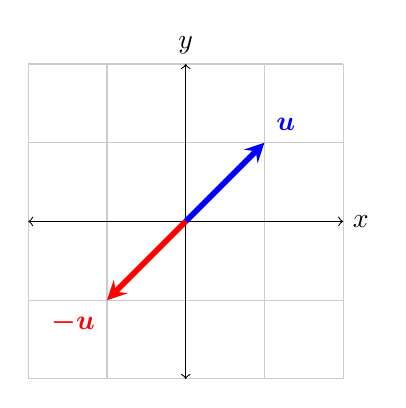
\begin{tikzpicture}
  \draw[thin,gray!40] (-2,-2) grid (2,2);
  \draw[<->] (-2,0)--(2,0) node[right]{$x$};
  \draw[<->] (0,-2)--(0,2) node[above]{$y$};
  \draw[line width=2pt,blue,-stealth](0,0)--(1,1)
        node[anchor=south west]{$\boldsymbol{u}$};
  \draw[line width=2pt,red,-stealth](0,0)--(-1,-1)
        node[anchor=north east]{$\boldsymbol{-u}$};
\end{tikzpicture}
\end{center}
\caption{\label{fig:vectors} Text size inside figure should be as big as
  caption's text. Text size inside figure should be as big as
  caption's text. Text size inside figure should be as big as
  caption's text. Text size inside figure should be as big as
  caption's text. Text size inside figure should be as big as
  caption's text. }
\end{figure}
%% %---------------------------


Here's a typical reference to a floating figure:
that instructs you to make sure that the size of the text within the
figures that you use is as big as (or bigger than) the size of the
text in the caption of the figures. Please do. Really.

In our case, we've explicitly drawn the figure inlined in latex, to
allow this tex file to cleanly compile. But usually, your figures will
reside in some file.pdf, and you'd include them in your document
with, say, \textbackslash{}includegraphics.

Lists are sometimes quite handy. If you want to itemize things, feel
free:

\begin{description}
  
\item[fread] a function that reads from a \texttt{stream} into the
  array \texttt{ptr} at most \texttt{nobj} objects of size
  \texttt{size}, returning returns the number of objects read.

\item[Fred] a person's name, e.g., there once was a dude named Fred
  who separated usenix.sty from this file to allow for easy
  inclusion.
\end{description}

\noindent
The noindent at the start of this paragraph in its tex version makes
it clear that it's a continuation of the preceding paragraph, as
opposed to a new paragraph in its own right.


\subsection{LaTeX-ing Your TeX File}
%-----------------------------------

People often use \texttt{pdflatex} these days for creating pdf-s from
tex files via the shell. And \texttt{bibtex}, of course. Works for us.

%-------------------------------------------------------------------------------
\section*{Acknowledgments}
%-------------------------------------------------------------------------------

The USENIX latex style is old and very tired, which is why
there's no \textbackslash{}acks command for you to use when
acknowledging. Sorry.

%-------------------------------------------------------------------------------
\section*{Availability}
%-------------------------------------------------------------------------------



\subsection{Migration protocol}
\label{sec:migrationprotocol}
We observe the lifetime of a migratable data structure from the point it is
created until after we finish migrating it to another node. Throughout the
lifetime of the object and during the migration process, there are certain
conditions that need to be satisfied by the application for the migration
operation to finish correctly. As discussed later in this section,
in many of these cases, forcing the application to satisfy low level conditions
cannot be completely achieved by the library and the responsibility of
conforming to these conditions will be left to the application.

of Slope at different stages during the above timeline.


\subsubsection{Object creation}
During this phase the source machine calls into the Slope library multiple
times, based on how many times memory allocation and deallocation is required.

\paragraph{Source} creates a migratable object. Let us call this object
the target object. Up until the point that
the source initiates the migration, all of the memory allocations of the target object
must happen through
Slope's custom memory allocator through allocation contexts as discussed in
The application must satisfy the memory allocation requirements discussed in

After the object is created the program will call the \texttt{run()} method
of the object, which may result in further calls to the memory allocator as
the object might need to allocate memory to process its incoming requests or
carry out the calls to its member functions. These new allocations will be
correctly picked up by Slope allocator given that allocation contexts are used
know which memory pages belong to the target object.

\subsubsection{Migration initiation}
The application logic decides that the target object must be migrated from the
source machine to the destination. This might happen because the source machine
is balancing out its load by offloading the object to the destination or because
this particular object will benefit from running on the destination machine
by being local to resources that are available there.

This is the first time that the destination
machine will need to know about the properties of the target object. Had the
source machine not initiated the migration, the destination machine would have
stayed unaware of the existence of this object.

\paragraph{Source}
initiates the migration by calling into Slope. From this point
on, the application instance on the source machine is neither allowed to
cause any memory to be allocated to the target object, nor can it deallocate any memory that
this object references. Each of these can result from calling member functions
of the target object which either deallocate Slope memory previously held by the
object, or create Slope memory allocation contexts from the object and
use them to allocate Slope memory for the object.

This means the underlying Slope memory owned by this object is now
fixed. The application can continue to read or write to the memory that the
object already owns, until further on in the process when it receives a
notification from the Slope library. This notification signals that source
machine no longer owns the object, prohibiting this machine from any
interaction with the target object, including reading from or writing to its
memory. This will be discussed in detail in the following sections.

Slope posts a send request to the QP that is shared
between the source and the destination, initiating the migration.
With this request, the source will include $n$ the total number of
memory pages that the target object references. Note that Slope requires the
memory pages owned by the target object to stay the same during the migration
process after a call which initiates the migration, which means $n$ will be
constant throughout the process.

\paragraph{Destination}
receives a migration request along with $n$, the number of memory pages that the
target object owns and therefore need to
be transferred. The destination then populates another QP shared with the source
with $n$ receive requests, each corresponding to one of the virtual memory pages
that underlie the target object. We switch to a different QP
to allow concurrent migrations to happen between pairs of nodes. The destination
then goes on to notify the source that it can receive the description of the $n$
pages. The destination needs to know the page addresses
to first create mappings for them and then pin them in physical memory so that their
physical address will stay the same throughout the migration, while the network
device writes to the pages by their physical address over DMA.

\paragraph{Source} receives the clear to send from the destination and sends the starting address
of each of the $n$ pages to the destination. 

\paragraph{Destination} waits for $n$ page addresses, and for each one of them, pins the
corresponding page in physical memory, so that the addresses that underlie the
target object can be used in RDMA read and write verbs. Notice how
``pro-active'' strategies which do not require knowledge of the page addresses
will not work, as pinning the
whole Slope memory in the physical memory will in the worst case, exhaust the
available physical memory on some nodes, and in the best case, result in large
amounts of wasted physical memory space. When the $n$ pages are pinned
and are ready to be the target of the RDMA verbs, the destination responds back,
signaling that it has pinned all of the required pages.

\subsubsection{Prefill}
The goal of the prefill phase is to warm up the destination machine's memory to
minimize the window of time during which none of the two participating machines
own the target object. No machine can read from or write to the object during
that time. Therefore a long window without no owners means a long throughput
and latency hiccup as the application does not make any progress.

During the prefill phase we copy the target object to the destination over RDMA.
What makes it different from simply transferring the contents of memory is that
during the prefill operation, the source is still allowed to write to
any location in the target object memory,
despite not having permission to change the memory layout of the object
in any way by allocating or deallocating memory. We optimistically do the above
transfer knowing that some of the pages might need to be retransferred as they
are written to by the source machine after they are sent to the destination.
We will refer to these pages as dirty pages. While pages can be
dirtied, we go through the prefill phase, hoping that one of the
machines (namely the source machine) will be able to partially function during
this phase, while dirtying a small percentage of the pages.

\paragraph{Source} will need to loop through the memory pages of the target
object to prepare them to be read safely by the network device. It will then
need to use RDMA WRITE to send them to the destination, but before it is ready
to go through these, it must put in place the means to detect the pages that
are dirtied. A page will be dirtied when a write takes place in it, after
it is sent to the destination.

\subparagraph{Dirty page detection:}
This will be done using memory mapping protections and manually
handling signals that
are raised as a consequence of accesses to the protected memory pages.

First, the source overrides the default behavior of handling the
\texttt{SIGSEGV} signal using a call to
\texttt{sigaction}, to prevent the program from terminating on invalid memory
references. It is important to keep in mind that \texttt{SIGSEGV} is delivered
to the \emph{same} thread whose current instruction reads or writes memory
from a page that does not have the required permissions.

To synchronize the access to the pages of the target object,
we set the protection flags of each page to \texttt{PROT\_READ} before sending
it over RDMA. This prevents any writes from happening while RDMA WRITE
is in progress. These writes will result in a \texttt{SIGSEGV} signal being
raised because of an invalid memory reference, and the thread will start
executing our custom \texttt{SIGSEGV} handler.

Inside the signal handler, we make note of the address the access
to which caused the signal to be raised. This can be found in the
\texttt{si\_addr} field from the
\texttt{struct {*}siginfo\_t} which is passed to the handler.
Assuming this is an address in a
page that the target object owns, we mark the page containing the address as
dirty. In the simplest case, the RDMA WRITE corresponding to this page has
previously finished. We update the protection flags of this page back
to \texttt{PROT\_READ | PROT\_WRITE}
to allow further writes to the addresses in this page to succeed.

Otherwise the RDMA WRITE is still in progress in which case we need to be
more careful. In this case we need to wait for the
RDMA WRITE to finish before adding the \texttt{PROT\_WRITE} permission flag to
the page. In our
implementation we use a conditioned shared mutex where the thread which carries
out the RDMA operations is the writer and the threads that may call into the
signal handler are potential readers. As a result, each thread will will block
inside the signal handler until
the address to which they are trying to write acquires the correct permission.
as each of them they fall into one of the above cases while Slope prefills a
page.


\subparagraph{Preparation:} At this point in the process, the source still
has ownership over the target object memory. This means we need to coordinate
the access to these pages to prevent simultaneous reads and writes. To do this,
the source uses \texttt{mprotect} to make the current page read-only.
Semantically, the application is still allowed to write to the current page,
except when the RDMA SEND is happening.

\subparagraph{Send:} Each page is posted to a data plane QP shared between the
source and the sink, to be written to its corresponding virtual address in
destination over RDMA. Notice that we do not put the \texttt{PROT\_WRITE} permission
of the current page back after the RDMA SEND finishes, as we need to
detect any future writes which will dirty the page.
However we do set a condition variable which a threads running the signal
handler will check to know whether or not it is clear to put the \texttt{PROT\_WRITE} flag back.
At any point in time the clean pages will have their condition variable unset,
which is how we distinguish between the dirty and clean pages.

One by one, the source prepares and writes each page that the target object
owns, using the above procedures and keeps track of which of them is dirtied
over time.

\subsubsection{Transfer of ownership}

Contrary to case of detecting the pages that become dirty, which can be done
as described above, prevention of this phenomenon cannot be dealt with this way.
For example we may try to set texttt{PROT\_NONE} permission on a page to
prevent accesses to it after we have started to send it to the destination.
The reason why this will not work will be discussed in the next section.


This cannot be correctly enforced by means such as setting the
\texttt{PROT\_NONE} on these pages. First, we might need multiple
\texttt{mprotect} calls to accomplish this if the pages are not adjacent,
meaning that we cannot assume the access to the object is ceased at a single
point in time. Furthermore even if we are able to take away the access to all
of the memory under the target object at once, if an application thread is
currently in the process of writing to the above memory, there is no right
action we can take from outside the application. For example this might have
been one write operation in the middle of a series of writes that the
application had been doing during the execution of a certain function. Therefore
from the standpoint of the library, we do not have enough information to deal
with cases similar to these, as aside from detecting the illegal writes, there
is no right action to take to remedy them.

\label{sec:transferownership}
At this point we are ready to turn the ownership over to the destination.
We also have to notify the application at the source to stop referencing the
target object for both reads and writes before we can proceed.

\paragraph{Destination} receives the completions for the prefill RDMA WRITEs.
That is because those WRITEs are done with immediate values which will results
in completion entries to be created for them. After the destination
receives the completion of the
last SEND, it will send a request back to the source, asking the source to
finally give up the ownership of the object.

\paragraph{Source} calls back to the application upon receiving the above
message to make sure the application will not reference the target object
for either of reads or writes after the callback returns. The application is
therefore responsible to block the callback an notifies all of its threads to
finish their ongoing operations on the target object. The application will
ideally transition to a ``pre-transfer'' mode after the initial migration
initiation. In this phase the application will try to do mostly read-only
accesses to avoid dirtying too many pages as this will cause the migration
to be done less efficiently with more pages that need to be transferred twice.
discuss how this model fits naturally in C++ programs.

After the application clears the migration, effectively promising to never
reference the target object again, Slope will use the dirty
page tracking data to identify the dirty pages and send their addresses
to the destination. This message will also hand over the ownership
of the target object to the destination.

\paragraph{Destination} is notified that it has been given the ownership of
the object and is clear to start the \texttt{run()} method of the object,
but also needs to re-pull the dirty pages whose address is attached to the
request since the contents of these pages on the destination machine are
outdated.
Slope starts the above two processes concurrently. The destination machine
first sets
\texttt{PROT\_READ | PROT\_WRITE} access for the clean pages and
\texttt{PROT\_NONE} for the dirty pages. We put the dirty page addresses into 
a priority queue and fetch them from the source machine in order, giving
precedence to the pages which result in a
\texttt{SIGSEGV} being raised at the destination from an access by the
application. This means that the page has \texttt{PROT\_NONE} permission set and
is immediately required by an application thread. When the page is pulled using
RDMA READ, the page mapping flags will be updated to include read and write
permissions and any thread waiting for those pages can proceed. This is done
similar to how we do the dirty page detection on the source machine which was
discussed earlier.

\subsubsection{Post-transfer}
After the transfer is done, the state of the application will be
indistinguishable from a situation where we allocated the target object on
the destination machine from the start, if we deal with one final housekeeping
task.

\paragraph{Destination} will notify the source that it has READ all of the
dirty pages and that it no longer needs the destination to keep the
pre-transfer content of the object memory.

\paragraph{Source} will wait to receive the above message at which point it
safely \texttt{munmap}s the memory underlying the ``old'' target object. At
this point the state on the source looks as if the said object had never existed
there.


\section{Conformance to C++ language terminologies}
\label{sec:conform}
e.g. const, mutable, const cast


\section{Optimizations and Corner cases}
e.g. have to send the location of the object itself also: from
which address to create the migration pointer.

USENIX program committees give extra points to submissions that are
backed by artifacts that are publicly available. If you made your code
or data available, it's worth mentioning this fact in a dedicated
section.

%-------------------------------------------------------------------------------
\bibliographystyle{plain}
\bibliography{\jobname}

%%%%%%%%%%%%%%%%%%%%%%%%%%%%%%%%%%%%%%%%%%%%%%%%%%%%%%%%%%%%%%%%%%%%%%%%%%%%%%%%
\end{document}
%%%%%%%%%%%%%%%%%%%%%%%%%%%%%%%%%%%%%%%%%%%%%%%%%%%%%%%%%%%%%%%%%%%%%%%%%%%%%%%%

%%  LocalWords:  endnotes includegraphics fread ptr nobj noindent
%%  LocalWords:  pdflatex acks
